\chapter{Literature Review and Background Theory}

\section{Twitter as an indicator}
\subsection{Fastest Finger Wins}

With the current speed of information distribution, financial markets react to new information quickly and prices adjust rapidly. This suggests markets are semi-strong efficient\cite{efficient_markets}, though the time frames have shortened considerably since the market theories were first proposed. Essentially, systematic traders don't just have to have the right trade, they have to make it before the rest of the market absorbs the information.

Even though online sources of news are typically trusted less than TV, radio and print\cite{modern_news}, the velocity of online news, especially from verified accounts means that it can be used as a fast source of information\cite{laney01controlling3v}. Scraping data from a wide variety of online sources posting corroborative stories improves the veracity\cite{laney01controlling3v}.

After a shock event, government agencies typically have access to the information first. They have the resources to dedicate to public warning systems which is not usually commercially viable\cite{earthquake_flow}. The government department then disseminates the information publicly and it is picked up by news agencies with their contacts. News agencies are likely to have this information before news outlets, as the latter typically purchases their news content from the former. These news agencies then distribute the information to the wider public.

The speed of this dissemination is currently being studied by academics. Kwak et al.\cite{Twitter_Kwak} looked at the dissemination of headline information on Twitter, with a tweet once re-tweeted, quickly reaching 1000 retweets. The one caveat they mentioned is that there is some level of homophily. Homophily is the predisposition of individuals to only interact with people similar to themselves. In the context of online dissemination of news about earthquakes, this is less of an issue, because earthquakes are universally covered by conservative and liberal newspapers, and in a wide variety of languages. This reinforces the assumption that once a news agency has picked up on an earthquake, it can be considered public knowledge.

The USGS has over 2,000 real-time sensors globally, calibrated to detect tremors. Despite this, there are many parts of the world not covered by their sensors\cite{usgs_stats}. In May 2008, an earthquake measuring 8.0 on the Richter scale struck the Sichuan region in China, and it was picked up by social media before the USGS's sensors. Currently, teams at USGS are researching the use of Twitter feeds as a secondary source to their sensors\cite{USGS_twitter}.

\subsection{Reading Tweets with NLP and NER}

Twitter particularly has drawn significant interest from both the academic community and financial market participants for its powers as a sentiment analysis tool. Many market data vendors, such as Bloomberg, offer data feeds of unstructured text, such as news headlines and Twitter streams\cite{bloomberg}. Different analysis approaches have been attempted such as hashtags, parts of speech and emoticons. Kouloumpis et al. found that hashtags and emoticons were useful approaches to the collection of training data for sentiment\cite{Twittersentiment}. They also found that using parts of speech was not.

Kireyev et al.\cite{Kireyev_Applications} examined some of the challenges associated with using micro-blogging sites such as Twitter. Specifically, the lack of detail and the casual format are two of the challenges mentioned. In this project, using official accounts of news sites, many of the issues with typos and colloquialisms are overcome as official accounts are more likely to use formal language, and be proof-read for spelling errors.

With the commercial applications derived from reading short form tweets, natural language processing (NLP), and more specifically named-entity recognition (NER) is a focus of many computer science departments\cite{polyglotner}\cite{ritter_nlp}\cite{stanford_ner}. Stanford University released a Java-based NER in 2005\cite{stanford_ner}, focusing on three classes; people, organisations and locations. This was released before Twitter was invented, and does not work well on the typical short-form text of 280 characters. Ritter et al.\cite{ritter_nlp} built a Twitter specific NER tool, which starts with parts of speech tagging before moving on to NER. More recently released (2015) is a multi-language python-based library called Polyglot\cite{polyglotner}. As well as parts of speech tagging, and NER, Polyglot takes advantage of distributed word representations (word embedding) to apply the same model to multiple languages.

These systems are invaluable to researchers looking to extract the relevant information from a large number of tweets quickly.

\pagebreak
\section{Classification based on Artificial Neural Networks}

\subsection{Machine Learning}

\subsubsection{Background}

Machine learning is an area of artificial intelligence that uses the power of modern computer science to apply statistical techniques in order to find an optimal solution to a problem\cite{understand_ml}. The statistical techniques applied can also allow a system to find meaningful patterns in complex data-sets\cite{intro_ml}.

Machine Learning doesn't require a programmer to provide detailed specifications of how the inputs map to the outputs, it merely provides the problem boundaries and allows the system to learn the mappings. This has allowed machine learning to replace expert systems in many applications\cite{Caudill_nn_primer}. Expert systems work best when the parameters of the problem have been rigorously studied and are both well known and widely accepted. In new areas, machine learning needs to be used, because there is no established body of work to draw upon \cite{intro_ml}. In the case of social media analysis, there is still much study to be done before definitive rule engines can be built.

\subsubsection{Machine Learning Algorithms}

Machine learning algorithms typically fall into one of three categories: supervised, unsupervised, and reinforcement learning\cite{Sutton:1998:IRL:551283}. In supervised learning, the system is fed both inputs and outputs, and it is able to judge how correct its model is as it learns\cite{intro_ml}. Essentially, the system is learning from experience. Two examples of supervised learning problems are regression, such as linear regression models, and classification, such as a decision tree. On the other hand, un-supervised learning only provides the input data\cite{Goodfellow_deeplearning}, and the algorithms are focused on finding patterns in the data, such as clustering algorithms. Reinforcement learning algorithms interact with the environment and make decisions based on the current status \cite{Sutton:1998:IRL:551283}.

Some other parameters to class learning algorithms are active vs passive learners or online vs batch learning protocols\cite{understand_ml}. Active learning algorithms are required to interact with the environment, while passive algorithms simply work with the data provided. Batch learning algorithms differ from online algorithms by having the opportunity to examine multiple inputs before being tested on the accuracy of conclusions.

The classification of tweets problem described in Chapter 1, is a classification problem which requires supervised passive learning. The training can be done in batches, and if implemented, can also learn online as new information is presented.

\subsection{Neural Network Setup}

\subsubsection{Input Selection}

Dr Robert Hecht-Nielsen\cite{Caudill_nn_primer} defined a neural network as \textit{``...a computing system made up of a number of simple, highly interconnected processing elements, which process information by their dynamic state response to external inputs.''}

The choice of inputs into this system is fundamental to the success of training the Neural Network. May et. al \cite{May_inputs} compared the selection of input variables for neutral networks with parametric empirical models. In parametric empirical models the inputs are based off the functional form of the model, but in neural networks, the inputs are selected from the available data.

They identified three issues when selecting variables for a neural network:
\begin{enumerate}
    \item[i] The available variables may be very large.
    \item[ii] There may be correlation between variables.
    \item[iii] Some of the variables may have no predictive power, and simply add noise in the system.
\end{enumerate}

Traditionally, selecting the inputs to help improve a model's predictive power focuses on these considerations \cite{Miller84variables}:

\begin{itemize}
    \item Relevance: There needs to be enough variables to have predictive power.
    \item Computational Effort: More variables increases computational burden
    \item Training Difficulty: Training becomes more difficult if redundancies need to be built in, or if some variables are irrelevant
    \item Dimensionality: As the model dimensions increase linearly, the problem domain increases exponentially.
    \item Comprehensibility: It is harder to deduce the relationships from studying the output model weights for a complex model.
\end{itemize}

Because tweets only contain 140 characters, the amount of information available is limited, which provides a natural limit to the number and type of variables.

\subsubsection{Network Topology} \label{subsubsec:topology}

Modern neural networks, also known as artificial neural networks, or sometimes, feed-forward neural networks, are made up of interconnected nodes. Figure~\ref{fig:SimpleNetwork} shows a simple  that each of the connections has a weight, and each of the nodes has an activation function\cite{intro_ml}. These nodes are divided into layers; the input layer, one or more hidden layers, and the output layer.

The input layer receives data from sources external to the system and presents a pattern to the neural network. The output layer is the predictions 
Most neural networks will only require one or two hidden layers\cite{Goodfellow_deeplearning}, and networks with more are known as deep networks. Each node within a layer will usually have the same activation function.

\begin{figure}[H]
\caption{A simple neural network with a single hidden layer}
\label{fig:SimpleNetwork}
\centering
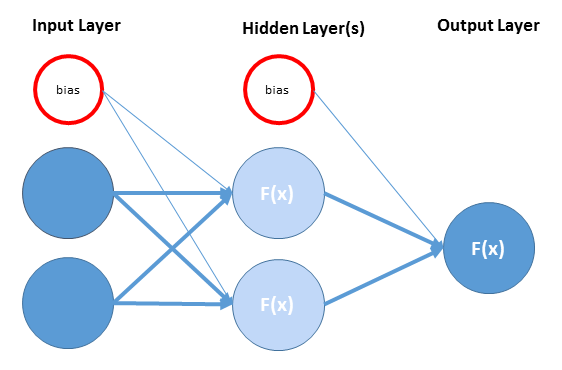
\includegraphics[width=1.0\textwidth]{Figures/SimpleANN.png}
\end{figure}

Often a Bias node is introduced to a connected network. The role of the bias unit is to act as an offset\cite{intro_ml}, shifting the activation function along the y-axis. Bias is implemented by default in Keras. There is an option to turn it off, but if it isn't required, a properly trained network will adjust the weights to zero.

As Stathakis observed\cite{hidden_layers}, traditional methods for identification of topology have been based on trial and error. Trial and error can be time-consuming and, without bounds, could delay more pressing research. The minimum required number of nodes in a network with a single hidden layer is usually the number of inputs\cite{Goodfellow_deeplearning}.

Sometimes, researchers have tried to stick to the following rules-of-thumb for their networks\cite{Saurabh_approx}:
\begin{itemize}
\item The number of hidden layer neurons are 2/3 (or 70\% to 90\%) of the size of the input layer. If this is insufficient then the number of hidden layer neurons can be added later on
\item The number of hidden layer neurons should be less than twice of the number of neurons in input layer.
\item The size of the hidden layer neurons is between the input size and the output size.
\end{itemize}

These mentioned approaches tend to lack sophistication, so some modern methods\cite{huang_two_layer} have tried to limit the maximum number of nodes required for a shallow network (two hidden layers), based on the number of outputs and samples presented. They proved that the number of hidden nodes that are enough to learn N samples with negligible error is given by:
\begin{equation}
    2\sqrt{\left(m+2\right)N} \label{eq:max_neurons}
\end{equation}

This can be further broken down into 
\begin{align}
    &1^{st} \text{Layer}: \sqrt{\left(m+2\right)N} + 2\sqrt{N/\left(m+2\right)} \label{eq:first_layer} \\
    &2^{nd} \text{Layer}: m\sqrt{N/\left(m+2\right)} \label{eq:second_layer}
\end{align}

Where m is the number of output neurons. Note that this does not take into consideration the number of inputs.
Other researchers have looked to use genetic algorithms\cite{learning_algorithm}\cite{hidden_layers} to calculate both the number of nodes and which layer to put them in. These approaches are trying to take the guesswork out of designing the topology of the network, which is designed to save researchers time in building and training their networks.

\subsubsection{Connections between nodes}

The nodes of different layers are connected to each other, as seen in Figure \ref{fig:SimpleNetwork}. There are different ways they can be connected, typically:

\begin{itemize}
    \item Dense / Fully connected
    \item Convolutional
    \item Pooling
    \item Normalisation
\end{itemize}

Densely connected layers are the most commonly used. Every input connects to a nodes, adjusted by a weight vector. The activation function is applied to the sum of these\cite{intro_ml}. The activation function can be linear or non-linear.

Convolutional layers are similar to dense layers. They use a similar matrix multiplication method on the input vector, but filters are used to take only a subset of the data\cite{hidden_layers} at a time. The activation function is usually a differentiable non-linear function. The purpose of convolutional layers in a deep feed-forward network is to reduce over-fitting. Convolutional layers assume that the inputs to the network are images. They are often used in alternating sequence with fully connected layers.

As well as convolutional layers, deep networks often contain pooling layers. In these deep networks, consecutive layers are activated by more complex functions, based off a larger number of inputs. A pooling layer effectively consolidates the outputs of a layer, so that the following layers don't need to perform as many operations. All the valid information is still transmitted, but these layers can help speed up training in large and complex networks\cite{hidden_layers}. Pooling layers are also usually used in networks that take images as inputs. They apply a function such as max or average to a group of outputs of a fully connected layer. This is only useful if those outputs are related in some way, such as in an image.

\begin{figure}[H]
\caption{Architecture of a CNN}
\label{fig:Convolutional}
\centering
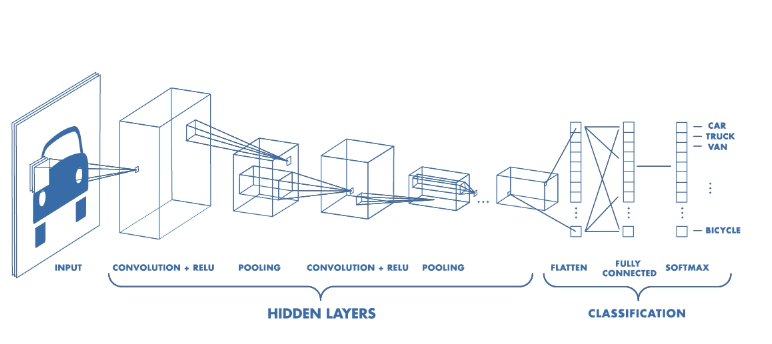
\includegraphics[width=1.0\textwidth]{Figures/convolutional.png}
\source{Medium\cite{conv_nn}}
\end{figure}

There are two main types of normalisation layers. Firstly, they can be used before the input layer for feature scaling\cite{LeCun_backprop}. Secondly, they can be used throughout the network to perform batch normalisation at hidden layers, if a network requires it.

As the inputs to the neural networks in this study are not images, convolutional and pooling layers have not been used. Fully connected and normalisation layers have both been used.

\subsubsection{Activation Functions}

The activation functions at each node should be differentiable semi-linear functions\cite{Rumelhart_error_propagation}. A semi-linear function is required to stop the system collapsing into a single layer linear function\cite{understand_ml}. The function must also be differentiable so that the system can efficiently update the weights through back-propagation of the errors through the network\cite{Rumelhart_error_propagation}. Some examples of common activation functions are sigmoid (Figure~\ref{fig:Sigmoid}), hyperbolic tangent (Tanh: Figure~\ref{fig:Tanh}), Softmax (Figure~\ref{fig:Softmax}) and rectified linear units (ReLU: Figure~\ref{fig:ReLU}).

Because of the way the sigmoid function forces scores to either zero or one, it is commonly used for classification problems. Tanh works in a similar way, and mathematically, Tanh is just a scaled version of sigmoid.

\begin{figure}[H]
\caption{Sigmoid Function}
\label{fig:Sigmoid}
\centering
\begin{equation}
A(x)=\frac{1}{1+e^{-x}}
\end{equation}
\begin{equation}
A'(x)=A(x)(1-A(x))
\end{equation}
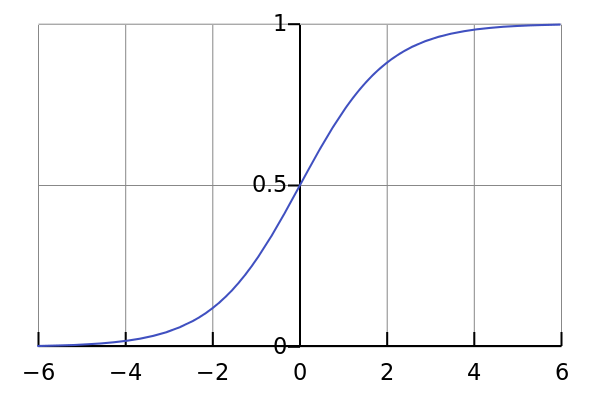
\includegraphics[width=0.6\textwidth]{Figures/Sigmoid2.png}
\source{Medium\cite{activ}}
\end{figure}

\begin{figure}[H]
\caption{Tanh Function}
\label{fig:Tanh}
\centering
\begin{equation}
A(x)=\frac{2}{1+e^{-2x}}-1
\end{equation}
\begin{equation}
A'(x)=1-A(x)^{2}
\end{equation}
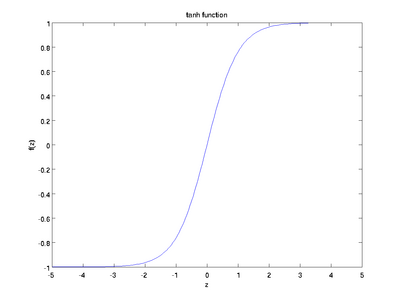
\includegraphics[width=0.6\textwidth]{Figures/Tanh.png}
\source{Medium\cite{activ}}
\end{figure}

Softmax function is also commonly used in classification problems, but usually when there are more than two possible classifications. This is known as multi-classification\cite{intro_ml}. Softmax is used in these cases because the sum of all probabilities will be equal to one, ensuring the outputs are classified distinctly.

\begin{figure}[H]
\caption{Softmax Function}
\label{fig:Softmax}
\centering
\begin{equation}
    A(x)_j = \displaystyle\frac{e^{x_j}}{\displaystyle\sum_{k=1}^{K} e^{x_k}} \text{for}~j = 1, ... , K
\end{equation}
\begin{equation}
    \frac{\partial}{\partial w_i }\sigma(j)=\sigma(j)\left(\delta _{ij}-\sigma(i) \right )x
\end{equation}
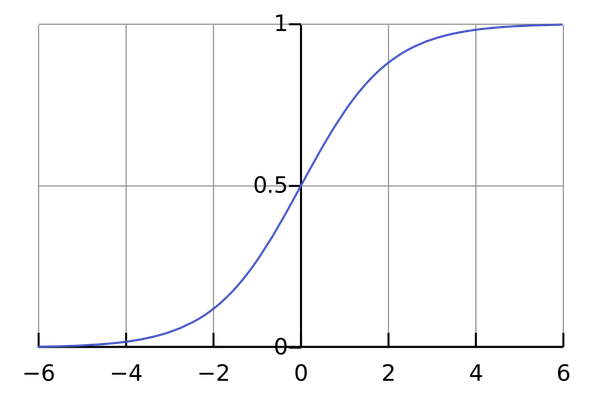
\includegraphics[width=0.6\textwidth]{Figures/Softmax.png}
\source{Introduction to Machine Learning\cite{intro_ml}}
\end{figure}

Where $x$ is an input in the vector $K$,  $j$ is the index of the input unit in $K$, and i is the index of the corresponding output unit. 

There are a number of issues with using these three as activation functions for hidden layers, such as the vanishing gradient problem\cite{LeCun_backprop} where the system stops learning if the gradient becomes too small. This is why, typically, ReLU is used as the activation function for hidden layers. It has also been shown\cite{Krizhevsky_neural} to be much faster in training many classification problems. However because the outputs of our classification problem are binary, ReLU is not appropriate for the output layer\cite{Rumelhart_error_propagation}.

\begin{figure}[H]
\caption{ReLU Function}
\label{fig:ReLU}
\centering
\begin{equation}
A(x)=max(0,x)
\end{equation}
\begin{equation}
A'(x)=1 \text{for} x>1, 0 \text{for} x<=0
\end{equation}
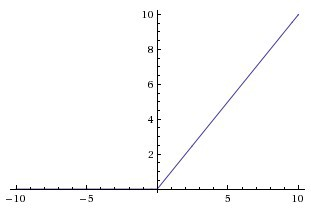
\includegraphics[width=0.6\textwidth]{Figures/ReLU.jpg}
\source{Data Science\cite{diff_activ}}
\end{figure}

From Figure \ref{fig:ReLU} the ReLU activation function returns zero for all negative values. Because the scale of these negative values can be important, especially for inverse relationships\cite{LeCun_backprop} a modified version of ReLU called Leaky ReLU is often used.

In leaky ReLU, the negative values are used, but scaled by a number $\alpha$. $\alpha$ is always smaller than one. It can be fixed, or varied during training. When $\alpha$ is randomly adjusted during training, it can help to avoid over fitting in deep networks\cite{fast_learning}.

\begin{figure}[H]
\caption{Leaky ReLU Function}
\label{fig:Leaky ReLU}
\centering
\begin{equation}
A(x)=\alpha x \text{ for } x<0, x \text{ for } x >=0
\end{equation}
\begin{equation}
A'(x)=1 \text{ for } x>1, \alpha \text{ for } x<=0
\end{equation}
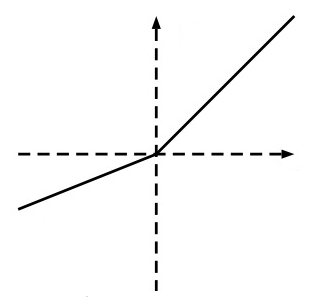
\includegraphics[width=0.6\textwidth]{Figures/LeakyReLU.png}
\source{Data Science\cite{activ}}
\end{figure}

\subsection{Training}

\subsubsection{Normalisation of inputs/outputs}\label{normalisation}

Before training a neural network, it is important to normalise the inputs and outputs. This will make it easier for the network to adjust the weights, and eventually make predictions\cite{Caudill_nn_primer}. Common normalisation techniques in neural networks are:

\begin{enumerate}
    \item Constant normalisation
    \item Min-Max normalisation
    \item Z-score normalisation
    \item Binary encoding
    \item Manhattan encoding
\end{enumerate}

Constant normalisation simply scales the input by a common divisor
\begin{equation}
z=\frac{x}{c}
\end{equation}

Min-Max normalisation forces all values to be within a certain range such as [0,1] or [-1,1]
\begin{equation}
z=\frac{x-min(x)}{[max(x)-min(x)]}
\end{equation}

Z-score normalisation assumes the input is normally distributed and uses the number of standard deviations from the mean as the input. This has the advantage of producing a mean of zero for the input, which LeCun et al.proved to improve convergence of weights\cite{LeCun_backprop} when training a neural network.
\begin{equation}
z=\frac{x_i-\mu}{\sigma}
\end{equation}

Binary encoding is common in neural networks. It is used in classification problems to produce a numeric representation of categories. For example True=1, False=0 or Boys=+1, Girls=-1.

Manhattan encoding is another example of representing classifications\cite{intro_ml}. Typically, 0s and 1s are used in a sequence to represent the classes. For example:
\begin{align*}
    \text{Hong Kong}&=[\;1\;0\;0\;0\;] \\
    \text{Japan}&=[\;0\;1\;0\;0\;] \\
    \text{South Korea}&=[\;0\;0\;1\;0\;] \\
    \text{Taiwan}&=[\;0\;0\;0\;1\;] \\
\end{align*}

This data pre-processing needs to be done before training to give the algorithms a better chance of finding the appropriate weights for a general solution.

\subsubsection{Network Hyper-parameters}\label{subsubsec:hyperparams}

In training a neural network, there are various hyper-parameters that need to be specified for the optimisation algorithm. Many of these parameters come from the generalised delta rule proposed by Rumelhart et al. in 1986\cite{Rumelhart_error_propagation}:
\begin{equation}
    \Delta w_{ij}(n+1)=\eta (\delta _{pj}o_{pi})+\alpha\Delta w_{ji}(n)
\end{equation}

where $\Delta w_{ij}$ is the change to be made to the weight from the $i$th to the $j$th unit following presentation of pattern $p$, $\delta_{pj}$ is the difference between the target input and the actual pattern produced for the $j$th component of the output pattern for pattern ~$p$, the subscript $n$ indexes the presentation number, $\eta$ is the learning rate, $o_{pj}$ is the $j$th element of the actual output pattern produced by the presentation of input pattern $p$, and $\alpha$ is a constant which determines the effect of past weight changes on the current direction of movement in weight space, also known as momentum.

Essentially, what this equation means, is that when a pattern is run through the current network, the result is compared with the target. Then the algorithm works its way back through the network, adjusting the weights on each connection by the difference of the target and observed patterns in proportion to the gradient of the activation function. This adjustment is modified by the learning rate. Also, because of the tendency of a system to fluctuate around the optimum, a momentum term is often included\cite{Rumelhart_error_propagation}. When used, momentum is usually from 0.5 to 0.9, and is it called Momentum Back Propagation (MoBP).

Sometimes, instead of using a momentum term, the learning rate can be decayed\cite{LeCun_backprop}. This will also help avoid the issue of fluctuation as the system will fluctuate less and less with further iterations. This is known as a Variable Learning Rate Back Propagation (VLBP).

When training a network, a variety of learning rates need to be tried. Common best practise is to narrow the search range through 

\begin{equation}
    lr_n = s g^{-n}
\end{equation}

where $lr$ is the learning rate, $s$ is the first learning rate, n is the iteration number, and g is the growth constant, typically 10\cite{Goodfellow_deeplearning}. After a range has been established, smaller a smaller space can be explored with a similarly methodical approach.

\subsubsection{Weights Initialisation}\label{subsec:weights}

To ensure training takes place, it is important to initialise the weights matrix. Rumelhart et al.\cite{Rumelhart_error_propagation} found that training would not occur if weights started at zero and chose random weights close to zero. If all weights are equal initially, every node will calculate the exact same signal. In order to break this symmetry, Hirose et al.\cite{Hirose_backprop} found that random weights limited to certain ranges would not converge:

\begin {table}[H]
\caption{Non-convergence according to Hirose et al.} \label{tab:initial_weights}
\begin{center}
    \begin{tabu}{||c c||} 
        \hline
        \rowfont[c]{\bfseries} Range of weights, ± & Percentage non-convergence  \\
        \hline\hline
        0.05 & 100 \\ \hline
        0.25 & 10 \\ \hline
        0.5 & 0 \\ \hline
        1 & 0 \\ \hline
        1.5 & 20 \\ \hline
        2.5 & 30 \\ \hline
        5 & 50 \\ \hline
    \end{tabu}
\source{Hirose et al.\cite{Hirose_backprop}}
\end{center}
\end{table}

LeCun et al.\cite{LeCun_backprop} furthered this research, suggesting that weights normalised around zero is appropriate. They proposed the range be based on the number of inputs to the layer:

\begin{equation}
    W_{ij} \sim U \left [  - \frac{1}{\sqrt n} , \frac{1}{\sqrt n}  \right ] \label{eqn:lecun1}
\end{equation}

where $W$ is the list of weights vectors, $U[-a, a]$ is the uniform distribution in the interval $(−a, a)$ and $n$ is the size of the previous layer (the number of columns of $W$).

The variance of weights in this case is:

\begin{equation}
    n Var[W] = \frac{1}{3}
\end{equation}

Which means that the variance of the back-propagated gradient is dependent on the layer. It follows that the gradient decreases with n, which increases the chance of the vanishing gradient problem with deeper neural networks\cite{Glorot_difficulties}. Glorot et al.suggested an alternative initialization procedure:

\begin{equation}
    W_{ij} \sim U \left [  - \frac{\sqrt{6}}{\sqrt{n_j + n_{j+1}}}, \frac{\sqrt{6}}{\sqrt{n_j + n_{j+1}}} \right ]    \label{eqn:glorot2}
\end{equation}

which uses the size of the current and following layer instead of the preceding layer. They proposed it maintained both activation variances and back-propagated variances. They called this normalized initialization and it has become the standard default in most neural network libraries such as Keras\cite{chollet2015keras}.

Further to this, to avoid the off chance of landing in a local minimum, it is best practice to run the same training parameters will different initial weights\cite{LeCun_backprop}.

% gradient descent vs ADAM or other optimisers

\subsubsection{Loss functions}\label{subsubsec:loss_func}

The loss function is what a system is trying to minimise overall, and is the judge of how effectively the network is trained. Loss functions typically fall into one of two categories, Regressive loss functions or Classification loss functions\cite{understand_ml}. The type of loss function selected, depends on the outputs required, and on the type of algorithm utilised.

Regressive loss functions are typically used when the target variable is continuous\cite{Nielsen_neuralnetworks}. An example of this is predicting a student's exam scores based on the number of hours studied and the number of hours slept. The most common one is mean squared error (MSE). Absolute error and smooth absolute error are commonly used as well. Mean squared error is calculated by:

\begin{equation}
    g\left ( y, \hat{y} \right )=\frac{1}{n}\sum{\left ( y_i - \hat{y}_i \right )^{2}}
\end{equation}

where $\hat{y}$ and $y$ represent the predicted and target values respectively. It penalises the distance between the predicted and target values.

When the target is a discrete value, classification loss functions are typically used\cite{Goodfellow_deeplearning}. The prediction represents the probability of that classification being true. Some common algorithms are:

\begin{enumerate}
    \item Binary Cross Entropy 
    \item Negative Log Likelihood
    \item Margin Classifier
    \item Soft Margin Classifier
\end{enumerate}

Binary Cross Entropy is the most common loss function for binary classification problems. It measures the divergence between two probability distributions. Binary Cross Entropy is calculated as:

\begin{equation}
    H_{{y}'}(y):=-\sum_{i}{y}'_i\log{y_i}
\end{equation}

where $y_i$ and ${y}'_i$ represent the predicted and target for class $i$, respectively. In the case of binary classification problems, the difference between the predicted probability and value representing the target classification.

Cross entropy is preferred to MSE for classification problems because it is more effective when trying to force the predictions to a distinct value\cite{Caudill_nn_primer}. With MSE, the weight adjustment factor gets smaller, as weights converge, but with cross entropy, the weight changes don't decrease.

\subsubsection{Model Fitting vs Over-fitting } \label{subsubsec:fitting}

When training a neural network, the intention is not to get 100\% accuracy on the training set, but to ensure the network is trained well enough generally to perform well on out-of-sample sets as well\cite{intro_ml}. When a system performs well on the training set, but poorly on the test set, this is known as over-fitting.

The difference between the model's predictions and the target, as calculated by the loss function, is called bias. The sensitivity of a model to small changes in the training set is called variance. High bias means the model has not yet been fully trained while high variance could mean the model has been over-fit.

\begin{figure}[H]
\caption{Bias vs Variance}
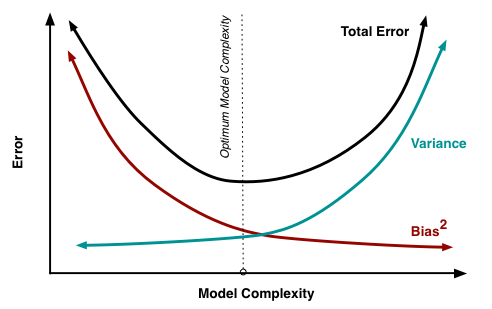
\includegraphics[width=0.9\textwidth]{Figures/biasvariance.png}
\source{Overfitting and Underfitting\cite{over_under}}
\end{figure}

There are various methods employed to avoid over-fitting, such as dropout or early stopping.
% regularisation, cross-validation, batch normalisation

Dropout refers to a practise in training a deep neural network, where some neurons are randomly selected to be ignored during a training run\cite{Goodfellow_deeplearning}. By dropping neurons during training, it reduces the co-dependency formed between the nodes and forces redundancy in the network\cite{Srivastava_dropout}. When training is complete, the 'dropped' nodes are added back for testing. According to Srivastava et al. this gives major improvements over other regularization methods because it is effectively averaging the predictions of all the thinned networks\cite{Srivastava_dropout}.

\begin{figure}[H]
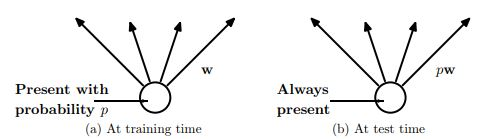
\includegraphics[width=0.9\textwidth]{Figures/Dropout.JPG}
\end{figure}

Nodes, and their connections are dropped based on a probability during training stages, but always present during testing. Whilst this is now a widely accepted practise for deep neural networks, for shallow neural networks, it is less effective\cite{Srivastava_dropout}.

For shallow networks, it is common to stop the training as soon as it has reached a certain level of accuracy, or after a certain number of epochs (training runs)\cite{Caudill_nn_primer}. This will have the effect of preventing over-fitting, as the network doesn't have the chance to perfectly fit the training set.

In early stopping, the data is typically divided into three sets\cite{girosi_neural}:
\begin{itemize}
    \item Training
    \item Validation
    \item Testing
\end{itemize}{}

The training set is the largest, it is usually 60\% to 70\% of total data. This is the set the model uses to adjust weights during stochastic gradient descent. The validation set is also used in testing, but it is used by the early stopping algorithm to check the effectiveness of training. If training has stagnated, and the model hasn't improved for a set number of iterations, the training is stopped early\cite{chollet2015keras}. The validation set needs to be at least 10\% of the testing set and is usually up to 20\%.

The testing set is used for the evaluation of the model. It was not used in testing and the model hasn't seen it before. This is the true test of the effectiveness of the model\cite{Prechelt97earlystopping}. As well as checking the loss function, the model can make predictions and check them against the expected values of the testing set.

As discussed by Ripley \cite{ripley2007pattern}, it is best practice to randomly select the the training, validation and testing sets from the total data, but it is important to ensure that the distribution is similar.

\subsection{Interpreting the output}

When the output produced by the neural network is a probability, between 0 and 1, the system needs a way of attributing this to a discrete classification. This requires a threshold level to be calculated.

The most common way of attributing this probability to a signal is through a receiver operating characteristics (ROC) graph\cite{Fawcett_threshold}. ROC graphs is a technique for organising, visualising and selecting classifiers based on their performance.

\begin{figure}[H]
\caption{Confusion matrix and commonly derived performance metrics}
\label{fig:ConfusionMatrix}
\centering
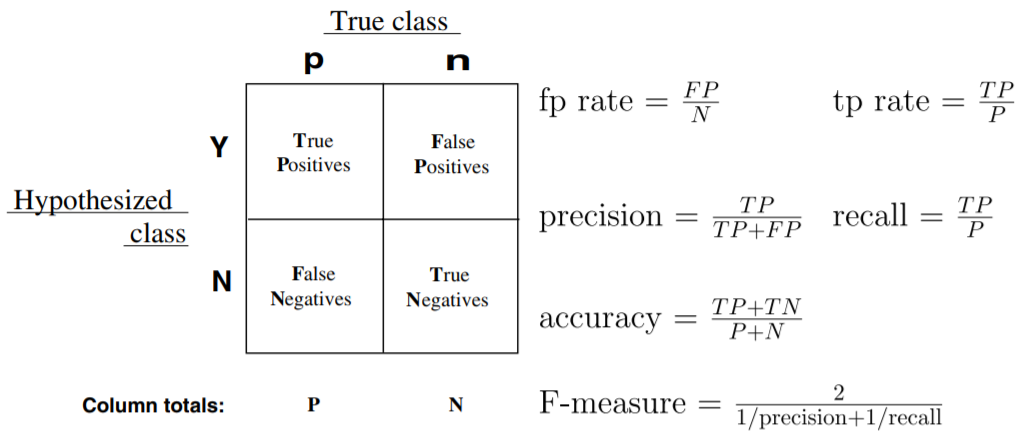
\includegraphics[width=1.0\textwidth]{Figures/ConfusionMatrix.png}
\source{Fawcett\cite{Fawcett_threshold}}
\end{figure}

Where fp rate is the false positive rate (type 1 errors) and tp rate is the true positive rate. Another common term is specificity, which is 1-fp rate. The precision is also often called the positive predictive value.

ROC graphs show the trade-off between the accurate predictions for true positives, and the type one errors potentially made. In an ROC graph, the fp rate from figure~\ref{fig:ConfusionMatrix} is plotted on the X axis and the tp rate is plotted on the Y axis. Points in the top left hand corner of the graph are the most desirable.

To compare points on this graph that are not directly related, area under curve (AUC) is calculated\cite{Guerriere_NN}. Because the axis are both proportions from 0 to 1, this calculated area will always be less than 1. The threshold that gives the highest AUC value according to equation \ref{eqn:auc} is the optimal threshold.

\begin{equation}\label{eqn:auc}
    AUC = \text{tp rate} * (1-\text{fp rate})
\end{equation}

This method of evaluation is commonly used in medical analysis, and other studies where the incidence rate of positives is expected to be low. However, this analysis required that a recommendation or decision be made. In financial services, unknown is also acceptable\cite{efficient_markets}.

This adjusts the calculation for tp to:

\begin{equation}\label{eqn:tp_adj}
    \text{tp rate} = \frac{TP}{P+UD}
\end{equation}

Where UD is the uncategorised responses. When this is calculated, the ROC can still be generated and the AUC can be calculated and compared.

\pagebreak
\section{Event Studies in Financial Markets}

\subsection{Asset classes}

An asset class is a term used to describe a group of securities with similar investment characteristics. These characteristics usually include risk profile, transaction costs, expected returns, and government regulations\cite{ross_corp}. The major asset classes are:

\begin{itemize}
    \item Equities
    \item Fixed Income
    \item Cash/FX
    \item Alternative Investments
\end{itemize}

The most popular asset class with retail investors is equities. Equities typically refers to common stock in a company listed on an exchange. But can also refer to preference shares, and exchange-traded funds (ETFs) and indices based on these. These instruments are only available to trade during specified market hours and usually not on weekends. Prices of these typically fluctuate more than fixed income and cash.

The other largest asset class for direct investment is fixed income. Fixed income refers to debt instruments issued by corporations, governments and related entities. It includes zero-coupon bonds and short-term money market instruments. These are typically traded over-the-counter (OTC) through an intermediary rather than on an exchange. Because bonds have seniority in the case of default and have a maturity date, they are usually considered a less risky investment than equities\cite{ross_corp}.

Cash includes all cash holdings which is considered to be zero-risk other than the inherent foreign exchange risk. Unlike other asset classes, FX markets are open 24 hours, 7 days a week. The foreign exchange market is by far the most liquid asset class by daily value traded\cite{ross_corp}.

Alternative investments is a large class, with many different sub-sections. These include commodities, direct real estate, art, private equity and more recently, crypto-currencies. Other than commodities, where secondary markets with regular trading contracts have been established, most alternative investments are considered illiquid, and not suitable for short-term trades\cite{efficient_markets}.

Most Equities, Fixed Income and FX instruments can be sold short directly\cite{ross_corp}. However, Market makers have established derivative markets on all of these asset classes including commodities. This allows investors to take positions on both the long and short sides of a trade\cite{agg_react} if they're not able to short the instrument directly.

Other than the commodities in the sections above, most of the instruments in each asset class belong to some kind of index. These indices are considered less risky to trade than single stocks because much of the company specific risk is diversified away.

Another option to trading a single instrument long or short, is a pair trade. A pair trade is when the investor goes long in one instrument, and short in another\cite{ross_corp}. The purpose of this is to gain exposure to some specific pricing differential while hedging some of the market risk inherent in a one-sided trade.

When trading financial instruments it is important to take into consideration transaction costs. The liquidity analysis required for these short term instruments is beyond the scope of this paper, but is important to note that this could negate any potential profits made from the trades.

\subsection{Event Study Methodology}

Testing for potential sources of alpha in financial markets is performed by both academics and market practitioners. This is especially true since Burton's work on random returns in 1973\cite{burton_random_walk}. With the power of modern computers, many researchers are using unsupervised learning. However, Keogh and Kasetty\cite{data_mining_Keogh} tested over 20 different data mining algorithms on over 50 different data sets with a view to verifying their utility. Their conclusion was that the data mining community needs to reduce the occurrence of implementation bias in their experiments and introduce objective benchmarks to verify algorithms.

Zhang and Zhou\cite{golden_nuggets} also examined the application of various data mining techniques to the finance industry. Specifically, they looked at Stock market predictions, portfolio management, bankruptcy prediction, foreign exchange markets, and fraud detection. They highlighted that the selection of appropriate inputs and algorithms, as well as model refinement and assessment are key components of event studies. Also, although neural network modelling is the most widely used method in data mining applications in finance, the optimal design of neural networks for various financial engineering problems remains open. At this stage they were not able to provide suggestions for appropriate algorithms and neural networks.

Because of these limitations, this report focuses on more traditional event study analysis using hypothesis testing. In more traditional event study analysis, first boundaries for the testing space must be established. Then, the space should be methodically searched for the results\cite{data_mining_Keogh}.

\subsection{Hypothesis testing}\label{subsec:hyp_test}

Hypothesis testing is a statistical approach to decision making.  Hypothesis testing first makes a tentative assumption about the expected results, and then uses logical or empirical tests to produce a statistical probability or confidence that the assumption is true or false.
%A hypothesis, as defined by the Merriam Webster dictionary is, \textit{"a tentative assumption made in order to draw out and test its logical or empirical consequences"}\cite{MerriamWebster2009}.

To conduct a hypothesis test, there are six main steps to follow\cite{black_stats}:
\begin{enumerate}
    \item Define Alternate Hypothesis and Null Hypothesis
    \item Decide on level of significance/confidence interval
    \item Calculate t-stat
    \item calculate p-value
    \item Make a decision on the null hypothesis
    \item Summarise conclusions based on decision
\end{enumerate}

A null hypothesis is the hypothesis assumed to be true, unless proven otherwise. The Alternate hypothesis is what the research is trying to prove. The alternate hypothesis is either:
\begin{itemize}
    \item The tested parameter is not equal to a certain value (a two sided test)
    \item The tested parameter is less than a certain value (left-tailed test)
    \item The tested parameter is greater than a certain value (right-tailed test)
\end{itemize}

The most commonly used significance level for event studies involving financial returns analysis is 95\%, which is approximately 2 standard deviations away from the mean in a normal distribution.

Because this work will involve forecasts, and the population's standard deviation is not known, the most appropriate statistic is the t-statistic\cite{black_stats}. The t-stat is based on the sample standard deviation:

\begin{align}\label{eq:tstat}
    t &= \sqrt{n}\frac{\Bar{x}-\mu}{s} \\
    df &= n-1 \nonumber
\end{align}

Where $t$ is the statistic calculated, $\Bar{x}$ is the sample mean, $s$ is the sample standard deviation and n is the number of observations. df refers to degrees of freedom. The formula in equation~\ref{eq:tstat} is for tests of a single population against a constant number, often zero. To test if the mean of two populations is significantly different, the formula is adjusted to include the distribution of the second population.

\begin{align}\label{eq:tstat_two}
    t&=\frac{\bar{Y_1}-\bar{Y_2}}{\sqrt{s_{1}^{2}/N_1+s_{2}^{2}/N_2}}
\end{align}

The p-value is calculated based on this statistic, and represents the probability of this being significant. P-values are compared to $\alpha$, which is calculated by:
\begin{equation*}
    \alpha = 1 - \text{Significance Level}
\end{equation*}

If the p-value is less than alpha, the null hypothesis is rejected. If the p-value is greater, the null hypothesis cannot be rejected. After the null hypothesis is rejected or not, the conclusions about the test can be discussed.

Because these are based on statistics, there is also a probability of error\cite{hypothesis}. There are two types of error; type 1 and type 2 errors. Type one error is false positives, where the test rejected a null hypothesis which is actually true. Type two error is a false negative, where the test did not reject the null hypothesis, when it is true.

Jegadeesh and Knaub\cite{jegadeesh_returns}\cite{knaub_hypothesis} both found evidence of excess returns in the stock markets using these methods. However, it should be noted, that they were both using end of day market data, unlike this report which looks at intra-day.

When performing any hypothesis test, it's also important to understand the assumptions behind the statistics\cite{black_stats}. When performing a t-test there are four main assumptions:

\begin{enumerate}
    \item The data is collected from a randomly selected and representative portion of the population.
    \item The data collected follows a continuous, and not discrete scale.
    \item The sample is a reasonably large size and follows a normal distribution.
    \item The variance of the sample is approximately equal to other samples from the same population.
\end{enumerate}

In order to have confidence of these holding true, the normality of a sample can be tested by measuring the skewness and kurtosis of the sample\cite{hypothesis}. These can be plotted and tested with regression analysis. Along with standard deviation, skewness and kurtosis explain the shape of the distribution. To test the assumption of normal distribution, skewness should be within $\pm$0.5 and kurtosis should be within range of $\pm$2.

To test that the sample is a reasonably large size, the below formula can be used:

\begin{equation} \label{eq:minpop}
    \text{Minimum Population} = \frac{Z^2 * \sigma (1- \sigma)}{me^2}
\end{equation}

Where $Z$ is the z-score of the confidence interval, $\sigma$ is the standard deviation of the sample, and $me$ is the margin of error accepted for the study\cite{black_stats}.

For a two-sample t-test, the above assumptions of normality also must hold true for both samples. Further to this, the standard deviations must be similar. This is tested by a F-test:

\begin{equation} \label{eq:fstat}
    F = \left( s^{2}_{1}/s^{2}_{2} \right)
\end{equation}

Where $F$ is taken from the critical value of the F distribution. For a two tailed F-test, it passes if $F$ is outside of the bounds calculated by the significance level chosen:

\begin{equation} \label{eq:fdist}
    F < F_{1 - \alpha/2,N_1 - 1,N_2 - 1}  \\
    or \nonumber\\
    F > F_{\alpha/2,N_1 - 1,N_2 - 1} \nonumber\\
\end{equation}

Even if a t-stat suggests the null hypothesis should be rejected, we cannot draw that conclusion if any of the assumptions are violated\cite{knaub_hypothesis}.

As well as tests that the returns are significantly different from zero, investors want to only invest where there is a reasonable risk/reward ratio. For analysing returns, the most common ratio is the sharpe ratio\cite{perf_eval}. This was first proposed by William Sharpe in 1966\cite{sharpe_perf} and describes returns in proportion to their risk.

\begin{equation}
    \text{Sharpe} = \frac{\Bar{r_p} - r_f}{\sigma _p}
\end{equation}

Where $r_p$ is the mean portfolio return, $r_f$ is the risk-free rate and $\sigma _p$ is the standard deviation of portfolio returns. Sharpe ratio greater than 1 is considered a "good" strategy\cite{ross_corp}. There are other measures such as Jensen's measure and Treynor ratio which are more equity specific and not applicable to other asset classes. Sharpe is widely used because it adjusts for a security's cost of capital through the risk free rate and can be applied to any publicly traded asset.

%Background:
%The goal is for your the contents of the literature review to be thorough with respect to the important statistical literature related to the problem.
% only want to cite publications that are related to your research.
%²  want to discuss how the cited literature is related to your research. That is,  want to refer to published research to motivate the originality and %relevance of your research.

